\subsection{Zernike modes PSFs Clustering}

	\subsubsection{UMAPS}
		
		Before clustering, UMAPS for flattened PSF matrices, flattend LP coefficients matrices and PL intensities are processed. The same configuration is used for the different number of modes.
		
		\begin{table}[h!]
			\centering
			\begin{tabular}{|c|c|c|c|}
				\hline
				\textbf{Dataset type} & \textbf{Number of neighbors} & \textbf{Min distance} & \textbf{Number of components} \\
				\hline
				PSF electric field & 500 & 0.5 & 1000 \\
				\hline
				PSF intensity & 500 & 0.5 & 1000 \\
				\hline
				Predicted PSF electric field & 500 & 0.5 & 1000 \\
				\hline
				Predicted PSF intensity & 500 & 0.5 & 1000 \\
				\hline
			\end{tabular}
		\caption{UMAP parameter configurations for PSFs}
		\end{table}
		
	
	\subsubsection{Clustering}
		
		Using DBSCAN I create clusters for the UMAP representations. In the tables CDM and CDV are Cluster Density Mean and Cluster Density Variance respectively.
		
		\paragraph{2 Zernike modes}:
		\begin{table}[h!]
			\centering
			\begin{tabular}{|c|c|c|c|c|c|c|}
				\hline
				\textbf{} & \textbf{$\epsilon$} & \textbf{neighbors} & \textbf{Clusters} & \textbf{CDM} & \textbf{CDV} & \textbf{Non noise points}\\
				\hline
				\textbf{Zernike coeffs} & 0.01 & 6 & 1535 & 41.12 & 92.65 & 63130 \\
				\hline
				\textbf{LP coeffs} & 0.99 & 5 & 1470 & 44.00 & 631.91 & 64686 \\
				\hline
				\textbf{PL fluxes} & 34.7 & 5 & 1431 & 45.46 & 739.78 & 65065 \\
				\hline
				\textbf{PSF electric field} & 0.154 & 5 & 1563 & 40.16 & 110.41 & 62774 \\
				\hline
				\textbf{PSF intensity} &  &  &  &  &  &  \\
				\hline
				\textbf{Pred PSF electric field} &  &  &  &  &  &  \\
				\hline
				\textbf{Pred PSF intensity} &  &  &  &  &  &  \\
				\hline
			\end{tabular}
		\caption{DBSCAN clustering for 2 Zernike modes datasets}
		\end{table}
		\FloatBarrier
		
		\paragraph{5 Zernike modes}:
		\begin{table}[h!]
			\centering
			\begin{tabular}{|c|c|c|c|c|c|c|}
				\hline
				\textbf{} & \textbf{$\epsilon$} & \textbf{neighbors} & \textbf{Clusters} & \textbf{CDM} & \textbf{CDV} & \textbf{Non noise points}\\
				\hline
				\textbf{Zernike coeffs} & 0.128 & 4 & 1448 & 38.10 & 1204.20 & 55183 \\
				\hline
				\textbf{LP coeffs} & 12.8 & 4 & 1551 & 34.98 & 1109.08 & 54265 \\
				\hline
				\textbf{PL fluxes} & 410 & 4 & 1500 & 35.54 & 1131.51 & 53324 \\
				\hline
				\textbf{PSF electric field} & 0.31 & 4 & 1587 & 29.02 & 862.14 & 46065 \\
				\hline
				\textbf{PSF intensity} &  &  &  &  &  &  \\
				\hline
				\textbf{Pred PSF electric field} &  &  &  &  &  &  \\
				\hline
				\textbf{Pred PSF intensity} &  &  &  &  &  &  \\
				\hline
			\end{tabular}
		\caption{DBSCAN Clustering for 5 Zernike modes datasets}
		\end{table}
		\FloatBarrier
		
		\paragraph{9 Zernike modes}:
		\begin{table}[h!]
			\centering
			\begin{tabular}{|c|c|c|c|c|c|c|}
				\hline
				\textbf{} & \textbf{$\epsilon$} & \textbf{neighbors} & \textbf{Clusters} & \textbf{CDM} & \textbf{CDV} & \textbf{Non noise points}\\
				\hline
				\textbf{Zernike coeffs} & 0.29 & 4 & 1428 & 30.30 & 953.86 & 43275 \\
				\hline
				\textbf{LP coeffs} & 26 & 4 & 1485 & 28.01 & 889.60 & 43397 \\
				\hline
				\textbf{PL fluxes} & 770 & 3 & 1616 & 31.85 & 1099.66 & 51474 \\
				\hline
				\textbf{PSF electric field} & 0.26 & 4 & 1459 & 30.45 & 894.56 & 44429 \\
				\hline
				\textbf{PSF intensity} &  &  &  &  &  &  \\
				\hline
				\textbf{Pred PSF electric field} &  &  &  &  &  &  \\
				\hline
				\textbf{Pred PSF intensity} &  &  &  &  &  &  \\
				\hline
			\end{tabular}
		\caption{DBSCAN Clustering for 9 Zernike modes datasets}
		\end{table}
		\FloatBarrier
		
		\paragraph{14 Zernike modes}:
		\begin{table}[h!]
			\centering
			\begin{tabular}{|c|c|c|c|c|c|c|}
				\hline
				\textbf{} & \textbf{$\epsilon$} & \textbf{neighbors} & \textbf{Clusters} & \textbf{CDM} & \textbf{CDV} & \textbf{Non noise points}\\
				\hline
				\textbf{Zernike coeffs} & 0.424 & 3 & 1639 & 25.89 & 880.85 & 42439 \\
				\hline
				\textbf{LP coeffs} & 35.5 & 3 & 1445 & 32.26 & 1064.67 & 46626 \\
				\hline
				\textbf{PL fluxes} & 950 & 3 & 1669 & 24.31 & 814.44 & 40577 \\
				\hline
				\textbf{PSF electric field} & 0.25 & 4 & 1607 & 27.05 & 831.31 & 44202 \\
				\hline
				\textbf{PSF intensity} &  &  &  &  &  &  \\
				\hline
				\textbf{Pred PSF electric field} &  &  &  &  &  &  \\
				\hline
				\textbf{Pred PSF intensity} &  &  &  &  &  &  \\
				\hline
			\end{tabular}
		\caption{DBSCAN Clustering for 14 Zernike modes datasets}
		\end{table}
		\FloatBarrier
		
		\paragraph{20 Zernike modes}:
		\begin{table}[h!]
			\centering
			\begin{tabular}{|c|c|c|c|c|c|c|}
				\hline
				\textbf{} & \textbf{$\epsilon$} & \textbf{neighbors} & \textbf{Clusters} & \textbf{CDM} & \textbf{CDV} & \textbf{Non noise points}\\
				\hline
				\textbf{Zernike coeffs} & 26.32 & 3 & 1431 & 26.32 & 841.71 & 37668 \\
				\hline
				\textbf{LP coeffs} & 40.05 & 3 & 1558 & 24.44 & 801.25 & 38079 \\
				\hline
				\textbf{PL fluxes} & 1010 & 3 & 1647 & 18.25 & 566.01 & 30067 \\
				\hline
				\textbf{PSF electric field} & 0.25 & 4 & 1621 & 27.86 & 852.32 & 34332 \\
				\hline
				\textbf{PSF intensity} &  &  &  &  &  &  \\
				\hline
				\textbf{Pred PSF electric field} &  &  &  &  &  &  \\
				\hline
				\textbf{Pred PSF intensity} &  &  &  &  &  &  \\
				\hline
			\end{tabular}
		\caption{DBSCAN Clustering for 20 Zernike modes datasets}
		\end{table}
		\FloatBarrier
		
		
	\subsubsection{Normalised Mutual Information}
		
		After running an NMI on the clusters these are the results:
		\begin{lstlisting}
	NMI from datasets created with 2 Zernike Modes
    		- LP coeffs and PL intensities:
    			0.8164576430824315
    		- LP coeffs and PSF: 
    			0.8175003226815989
    		- PL intensities and PSF:
    			0.7994322323774545
    		- LP coeffs and predicted PSF: 
    			0.8175646434293075
    		- PL intensities and predicted PSF: 
    			0.7983573747301721
    		- Predicted PSF and original PSF: 
    			0.8095814407687527
    				
	NMI from datasets created with 5 Zernike Modes
    		- LP coeffs and PL intensities: 
    			0.2546247849754754
    		- LP coeffs and PSF clusters: 
    			0.2761463896986409
    		- PL intensities and PSF clusters:
    			0.2169490063500632
    		- LP coeffs and predicted PSF clusters: 
    			0.28175438653504503
    		- PL intensities and predicted PSF clusters: 
    			0.21635800151194817
    		- Predicted PSF and original PSF clusters: 
    			0.5464235488639057

	NMI from datasets created with 9 Zernike Modes
    		- LP coeffs and PL intensities: 
    			0.19594140953604774
    		- LP coeffs and PSF clusters: 
    			0.19331293998931096
    		- PL intensities and PSF clusters: 
    			0.14033346512809078
    		- LP coeffs and predicted PSF clusters: 
    			0.18823201153015062
    		- PL intensities and predicted PSF clusters: 
    			0.13583799714028102
    		- Predicted PSF and original PSF clusters: 
    			0.4208027610913512

	NMI from datasets created with 14 Zernike Modes
		- LP coeffs and PL intensities: 
			0.2061877271415178
		- LP coeffs and PSF clusters: 
			0.22489998453619262
   		- PL intensities and PSF clusters: 
   			0.15638010188248286
   		- LP coeffs and predicted PSF clusters: 
    			0.22450523757936153
    		- PL intensities and predicted PSF clusters: 
    			0.15124830319698243
    		- Predicted PSF and original PSF clusters: 
    			0.3978566533293418

	NMI from datasets created with 20 Zernike Modes
    		- LP coeffs and PL intensities:
    			0.15590863566718433
    		- LP coeffs and PSF clusters: 
    			0.2096232888801945
    		- PL intensities and PSF clusters: 
    			0.11871048630190495
    		- LP coeffs and predicted PSF clusters: 
    			0.20997226177915623
    		- PL intensities and predicted PSF clusters: 
    			0.1269907541345761
    		- Predicted PSF and original PSF clusters: 
    			0.2983128702057625
	\end{lstlisting}
	
		\begin{itemize}
			\item There is a stronger relationship between LP coefficients and PL outputs than PSF to LP coefficients.
			\item The relationship between PSF and PL outputs is the weakest.
			
		\end{itemize}
		
		\begin{figure*}[ht!]
			\centering
			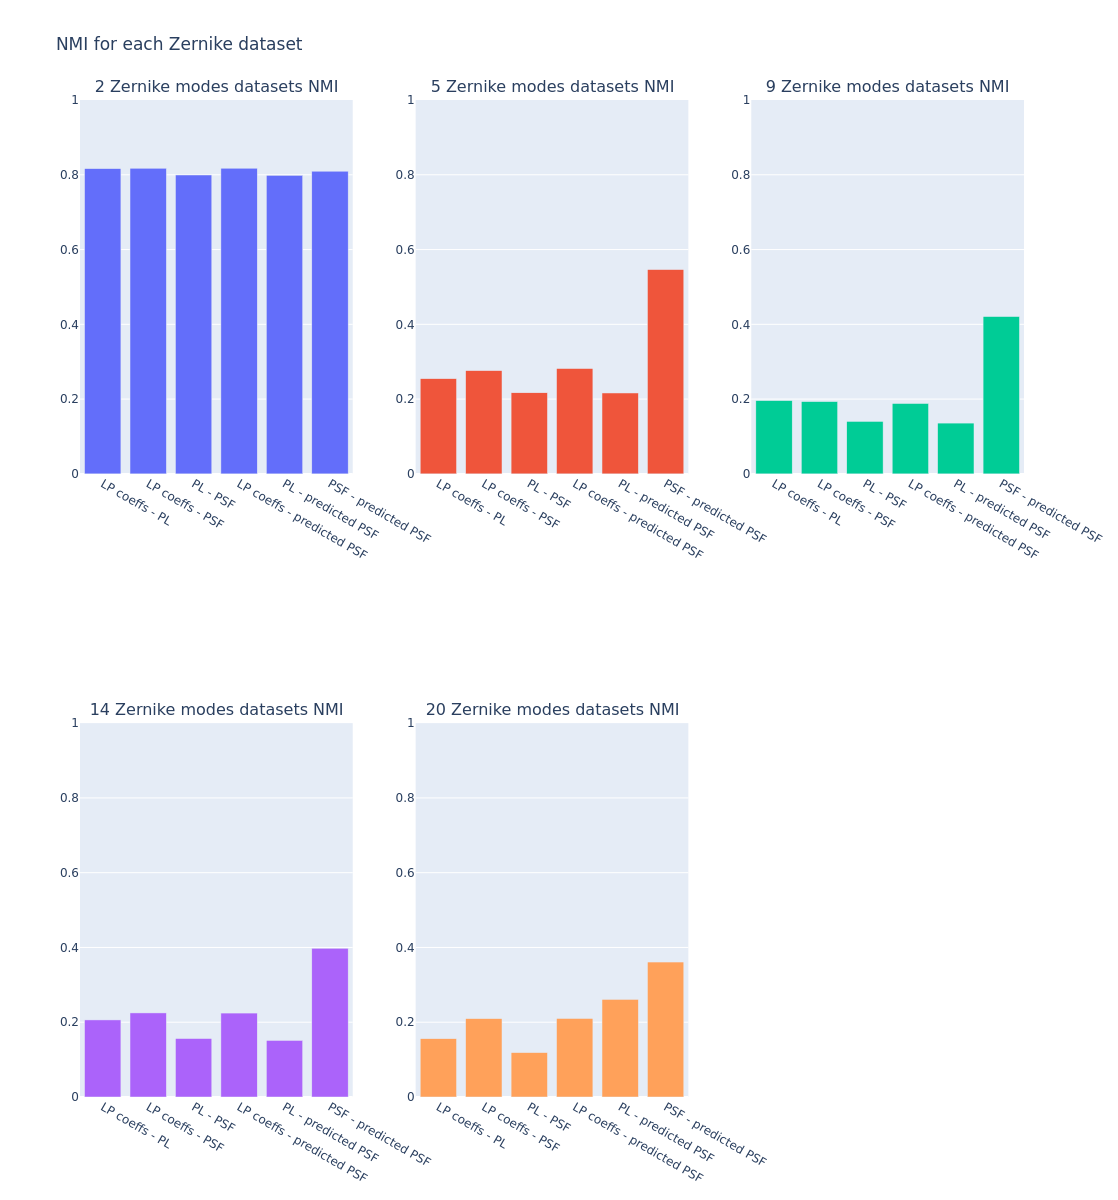
\includegraphics[width=0.7\textwidth]{pid-separatednmizernike.png}
			\caption{NMI for each of the Zernike related datasets}
		\end{figure*}